\documentclass{beamer}
\usetheme[faculty=law]{fibeamer}
\usepackage[utf8]{inputenc}
\usepackage[main=english]{babel}
\title{Cancer Detection} %% that will be typeset on the
\subtitle{An introduction to cancer detection using deep learning} %% title page.
\author{Mahdi Lotfi \\ Erfan Momeni \\ Araz Abedini \\ Matin Ghanbari}
%% These additional packages are used within the document:
\usepackage{ragged2e}  % `\justifying` text
\usepackage{booktabs}  % Tables
\usepackage{tabularx}
\usepackage{tikz}      % Diagram
\usetikzlibrary{calc, shapes, backgrounds}
\usepackage{epigraph}
\usepackage{amsmath, amssymb}
\usepackage{url}       % `\url`s
\usepackage{listings}  % Code listing
\begin{document}
  % \shorthandoff{-}
  \frame[c]{\maketitle}
  \AtBeginSection[]{% Printt an outline at the beginning of sections
    \begin{frame}<beamer>
      \frametitle{Outline for Section \thesection}
      \tableofcontents[currentsection]
    \end{frame}}

    \section{Machine Learning}
    \subsection{What Is Machine Learning}
    \begin{frame}[t]{Machine Learning}
      \framesubtitle{a slightly general definition}%
      \begin{tikzpicture}[overlay,remember picture]
        \node[anchor=south east,xshift=-30pt,yshift=35pt]
          at (current page.south east) {
            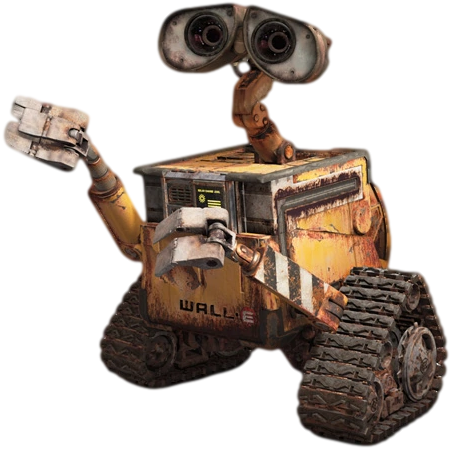
\includegraphics[width=35mm]{resources/wall-e}
          };
      \end{tikzpicture}%
      \begin{quote}
        field of study that gives computers the ability to learn without being explicitly programmed.
        \hfill {\tiny —Arthur Samuel, 1959}
      \end{quote}
      Machine Learning is the science (and art) of programming computers so they can \textit{learn from data}. \\
      \vspace{8mm}
      \parbox{0.55\textwidth}{
      Your spam filter is a Machine Learning program that, given examples of spam emails and examples of regular emails, can learn to flag spam.
      }
    \end{frame}
    \subsection{Types of Learning}
    \begin{frame}[label=lists]{Types of Machine Learning Systems}
      \framesubtitle{it is useful to classify ML algorithms in broad categories}
      \begin{columns}[onlytextwidth]
        \column{.5\textwidth}
          \begin{itemize}
            \item Nulla nec lacinia odio. Curabitur urna tellus.
            \begin{itemize}
              \item Fusce id sodales dolor. Sed id metus dui.
              \begin{itemize}
                \item Cupio virtus licet mi vel feugiat.
              \end{itemize}
            \end{itemize}
          \end{itemize}
        \column{.5\textwidth}
          \begin{enumerate}
            \item Donec porta, risus porttitor egestas scelerisque video.
            \begin{enumerate}
              \item Nunc non ante fringilla, manus potentis cario.
              \begin{enumerate}
                \item Pellentesque servus morbi tristique.
              \end{enumerate}
            \end{enumerate}
          \end{enumerate}
      \end{columns}
      \bigskip
      \justifying
      {\uselanguage{english}The quick, brown fox jumps over a lazy
      dog. DJs flock by when MTV ax quiz prog. “Now fax quiz Jack!”}
    \end{frame} 

    \begin{frame}{Artificial Intelligence Hierarchy}
        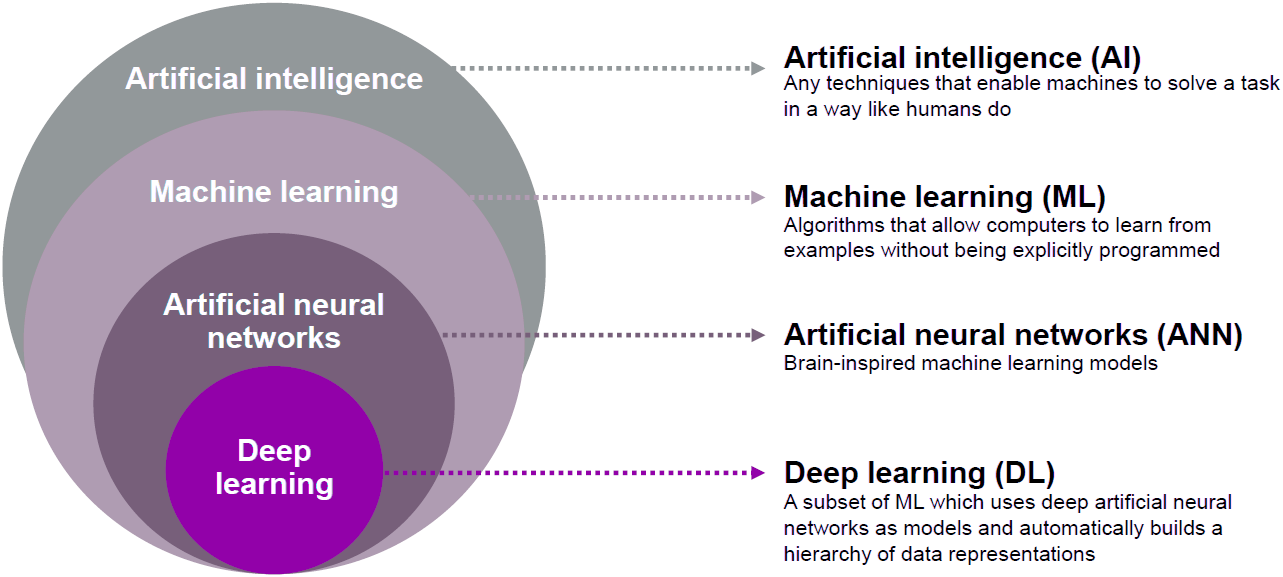
\includegraphics{resources/hierarchy}
    \end{frame}
    \begin{frame}[label=simmonshall]{Text blocks}
      \framesubtitle{In plain, example, and \alert{alert} flavour}
      \alert{This text} is highlighted.

      \begin{block}{A plain block}
        This is a plain block containing some \alert{highlighted text}.
      \end{block}
      \begin{exampleblock}{An example block}
        This is an example block containing some \alert{highlighted text}.
      \end{exampleblock}
      \begin{alertblock}{An alert block}
        This is an alert block containing some \alert{highlighted text}.
      \end{alertblock}
    \end{frame}

    \begin{frame}[label=proof]{Definitions, theorems, and proofs}
      \framesubtitle{All integers divide zero}
      \begin{definition}
        $\forall a,b\in\mathds{Z}: a\mid b\iff\exists c\in\mathds{Z}:a\cdot c=b$
      \end{definition}
      \begin{theorem}
        $\forall a\in\mathds{Z}: a\mid 0$
      \end{theorem}
      \begin{proof}[Proof\nopunct]
        $\forall a\in\mathds{Z}: a\cdot 0=0$
      \end{proof}
    \end{frame}

    \subsection{Deep Learning}
    
    \begin{frame}[t]{Representation Learning}
      \framesubtitle{find best representation of our data}%
      \begin{tikzpicture}[overlay,remember picture]
        \node[anchor=south east,xshift=-30pt,yshift=35pt]
          at (current page.south east) {
            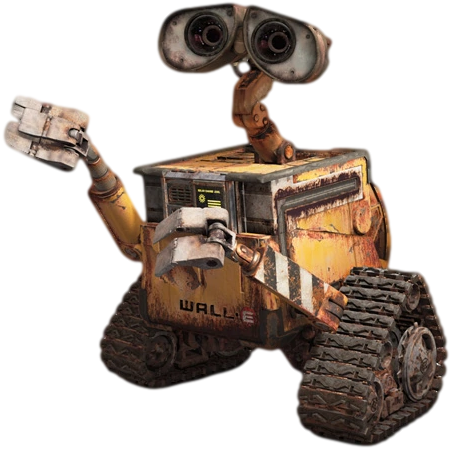
\includegraphics[width=35mm]{resources/wall-e}
          };
      \end{tikzpicture}%
      \begin{quote}
        field of study that gives computers the ability to learn without being explicitly programmed.
        \hfill {\tiny —Arthur Samuel, 1959}
      \end{quote}
      Machine Learning is the science (and art) of programming computers so they can \textit{learn from data}. \\
      \vspace{8mm}
      \parbox{0.55\textwidth}{
      Your spam filter is a Machine Learning program that, given examples of spam emails and examples of regular emails, can learn to flag spam.
      }
    \end{frame}

    \begin{frame}[t]{Deep Learning}
      \framesubtitle{a slightly general definition}%
      \begin{tikzpicture}[overlay,remember picture]
        \node[anchor=south east,xshift=-30pt,yshift=35pt]
          at (current page.south east) {
            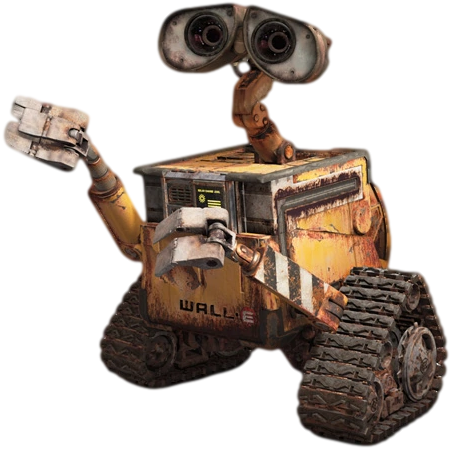
\includegraphics[width=35mm]{resources/wall-e}
          };
      \end{tikzpicture}%
      \begin{quote}
        field of study that gives computers the ability to learn without being explicitly programmed.
        \hfill {\tiny —Arthur Samuel, 1959}
      \end{quote}
      Machine Learning is the science (and art) of programming computers so they can \textit{learn from data}. \\
      \vspace{8mm}
      \parbox{0.55\textwidth}{
      Your spam filter is a Machine Learning program that, given examples of spam emails and examples of regular emails, can learn to flag spam.
      }
    \end{frame}

    \begin{frame}[label=math]{Numerals and Mathematics}
      \framesubtitle{Formulae, equations, and expressions}
      \begin{columns}[onlytextwidth]
        \column{.20\textwidth}
          1234567890
        \column{.20\textwidth}
          \oldstylenums{1234567890}
        \column{.20\textwidth}
          $\hat{x}$, $\check{x}$, $\tilde{a}$,
          $\bar{a}$, $\dot{y}$, $\ddot{y}$
        \column{.40\textwidth}
          $\int \!\! \int f(x,y,z)\,\mathsf{d}x\mathsf{d}y\mathsf{d}z$
      \end{columns}
      \begin{columns}[onlytextwidth]
        \column{.5\textwidth}
          $$\frac{1}{\displaystyle 1+
            \frac{1}{\displaystyle 2+
            \frac{1}{\displaystyle 3+x}}} +
            \frac{1}{1+\frac{1}{2+\frac{1}{3+x}}}$$
        \column{.5\textwidth}
          $$F:\left| \begin{array}{ccc}
          F''_{xx} & F''_{xy} &  F'_x \\
          F''_{yx} & F''_{yy} &  F'_y \\
          F'_x     & F'_y     & 0
          \end{array}\right| = 0$$
      \end{columns}
      \begin{columns}[onlytextwidth]
        \column{.3\textwidth}
          $$\mathop{\int \!\!\! \int}_{\mathbf{x} \in \mathds{R}^2}
          \! \langle \mathbf{x},\mathbf{y}\rangle\,\mathsf{d}\mathbf{x}$$
        \column{.33\textwidth}
          $$\overline{\overline{a\alpha}^2+\underline{b\beta}
           +\overline{\overline{d\delta}}}$$
        \column{.37\textwidth}
          $\left] 0,1\right[ + \lceil x \rfloor - \langle x,y\rangle$
      \end{columns}
      \begin{columns}[onlytextwidth]
        \column{.4\textwidth}
          \begin{eqnarray*}
           e^x &\approx& 1+x+x^2/2! + \\
             && {}+x^3/3! + x^4/4!
          \end{eqnarray*}
        \column{.6\textwidth}
          $${n+1\choose k} = {n\choose k} + {n \choose k-1}$$
      \end{columns}
    \end{frame}

    \begin{frame}[label=figs1]{Figures}
      \framesubtitle{Tables, graphs, and images}
      \begin{table}[!b]
        {\carlitoTLF % Use monospaced lining figures
        \begin{tabularx}{\textwidth}{Xrrr}
          \textbf{Faculty} & \textbf{With \TeX} & \textbf{Total} &
          \textbf{\%} \\
          \toprule
          Faculty of Informatics       & 1\,716  & 2\,904  &
          59.09 \\% 1433
          Faculty of Science           & 786     & 5\,275  &
          14.90 \\% 1431
          Faculty of $\genfrac{}{}{0pt}{}{\textsf{Economics and}}{%
          \textsf{Administration}}$    & 64      & 4\,591  &
          1.39  \\% 1456
          Faculty of Arts              & 69      & 10\,000 &
          0.69  \\% 1421
          Faculty of Medicine          & 8       & 2\,014  &
          0.40  \\% 1411
          Faculty of Law               & 15      & 4\,824  &
          0.31  \\% 1422
          Faculty of Education         & 19      & 8\,219  &
          0.23  \\% 1441
          Faculty of Social Studies    & 12      & 5\,599  &
          0.21  \\% 1423
          Faculty of Sports Studies    & 3       & 2\,062  &
          0.15  \\% 1451
          \bottomrule
        \end{tabularx}}
        \caption{The distribution of theses written using \TeX\ during 2010--15 at MU}
      \end{table}
    \end{frame}
    \begin{frame}[label=figs2]{Figures}
      \framesubtitle{Tables, graphs, and images}
      \begin{figure}[b]
        \centering
        % Flipping a coin
        % Author: cis
        \tikzset{
          head/.style = {fill = none, label = center:\textsf{H}},
          tail/.style = {fill = none, label = center:\textsf{T}}}
        \scalebox{0.65}{\begin{tikzpicture}[
            scale = 1.5, transform shape, thick,
            every node/.style = {draw, circle, minimum size = 10mm},
            grow = down,  % alignment of characters
            level 1/.style = {sibling distance=3cm},
            level 2/.style = {sibling distance=4cm},
            level 3/.style = {sibling distance=2cm},
            level distance = 1.25cm
          ]
          \node[shape = rectangle,
            minimum width = 6cm, font = \sffamily] {Coin flipping}
          child { node[shape = circle split, draw, line width = 1pt,
                  minimum size = 10mm, inner sep = 0mm, rotate = 30] (Start)
                  { \rotatebox{-30}{H} \nodepart{lower} \rotatebox{-30}{T}}
           child {   node [head] (A) {}
             child { node [head] (B) {}}
             child { node [tail] (C) {}}
           }
           child {   node [tail] (D) {}
             child { node [head] (E) {}}
             child { node [tail] (F) {}}
           }
          };

          % Filling the root (Start)
          \begin{scope}[on background layer, rotate=30]
            \fill[head] (Start.base) ([xshift = 0mm]Start.east) arc (0:180:5mm)
              -- cycle;
            \fill[tail] (Start.base) ([xshift = 0pt]Start.west) arc (180:360:5mm)
              -- cycle;
          \end{scope}

          % Labels
          \begin{scope}[nodes = {draw = none}]
            \path (Start) -- (A) node [near start, left]  {$0.5$};
            \path (A)     -- (B) node [near start, left]  {$0.5$};
            \path (A)     -- (C) node [near start, right] {$0.5$};
            \path (Start) -- (D) node [near start, right] {$0.5$};
            \path (D)     -- (E) node [near start, left]  {$0.5$};
            \path (D)     -- (F) node [near start, right] {$0.5$};
            \begin{scope}[nodes = {below = 11pt}]
              \node [name = X] at (B) {$0.25$};
              \node            at (C) {$0.25$};
              \node [name = Y] at (E) {$0.25$};
              \node            at (F) {$0.25$};
            \end{scope}
          \end{scope}
        \end{tikzpicture}}
        \caption{Tree of probabilities -- Flipping a coin\footnote[frame]{%
          A derivative of a diagram from \url{texample.net} by cis, CC BY 2.5 licensed}}
      \end{figure}
    \end{frame}

    \defverbatim[colored]\sleepSort{
      \begin{lstlisting}[language=C,tabsize=2]
  #include <stdio.h>
  #include <unistd.h>
  #include <sys/types.h>
  #include <sys/wait.h>

  // This is a comment
  int main(int argc, char **argv)
  {
          while (--c > 1 && !fork());
          sleep(c = atoi(v[c]));
          printf("%d\n", c);
          wait(0);
          return 0;
  }
    \end{lstlisting}}
    \begin{frame}{Code listings}{An example source code in C}
      \sleepSort
    \end{frame}

    \subsection{Convolutional Neural Networks}
    \begin{frame}[label=citations]{Citations}
      \framesubtitle{\TeX, \LaTeX, and Beamer}

      \justifying\TeX\ is a programming language for the typesetting
      of documents. It was created by Donald Erwin Knuth in the late
      1970s and it is documented in \emph{The \TeX
      book}~\cite{knuth84}.

      In the early 1980s, Leslie Lamport created the initial version
      of \LaTeX, a high-level language on top of \TeX, which is
      documented in \emph{\LaTeX : A Document Preparation
      System}~\cite{lamport94}. There exists a healthy ecosystem of
      packages that extend the base functionality of \LaTeX;
      \emph{The \LaTeX\ Companion}~\cite{MG94} acts as a guide
      through the ecosystem.

      In 2003, Till Tantau created the initial version of Beamer, a
      \LaTeX\ package for the creation of presentations. Beamer is
      documented in the \emph{User's Guide to the Beamer
      Class}~\cite{tantau04}.
    \end{frame}

    \section{Cancers}
    \subsection{What Is Cancer ?!}
    \begin{frame}[t]{What Is Cancer ?}
      
      \justifying\ Cancer is a disease in which some of the body’s cells grow uncontrollably and spread to other parts of the body. 
      You are made up of trillions of cells that over your lifetime normally grow and divide as needed. When cells are abnormal or get old, they usually die. Cancer starts when something goes wrong in this process.
      \vspace{8mm}
      
    \begin{tikzpicture}[overlay,remember picture]
      \node[anchor=south east,xshift=-90pt,yshift=20pt]
        at (current page.south east) {
          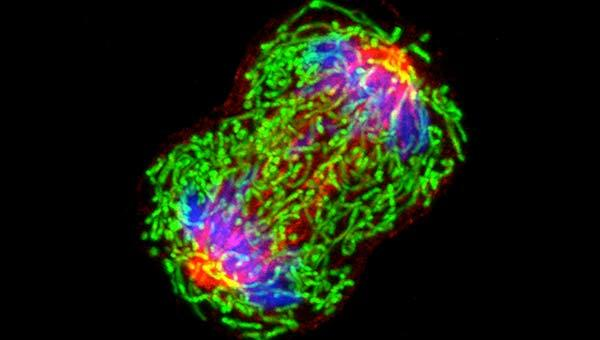
\includegraphics[width=55mm]{resources/dividing-breast-cancer-cell-article-only}
        };
    \end{tikzpicture}%
    \end{frame}
    \subsection{Types of Cancers}

    \begin{frame}[t]{Types of Cancers}
      Four main types of cancer are:
      \newline
      \begin{columns}[onlytextwidth]
        \column{.5\textwidth}
          \begin{itemize}
            \item Carcinomas
            \item Sarcomas
            \item Leukemias
            \item Lymphomas
            \end{itemize}
      \end{columns}
      
    \begin{tikzpicture}[overlay,remember picture]
      \node[anchor=south east,xshift=-250pt,yshift=20pt]
        at (current page.south east) {
          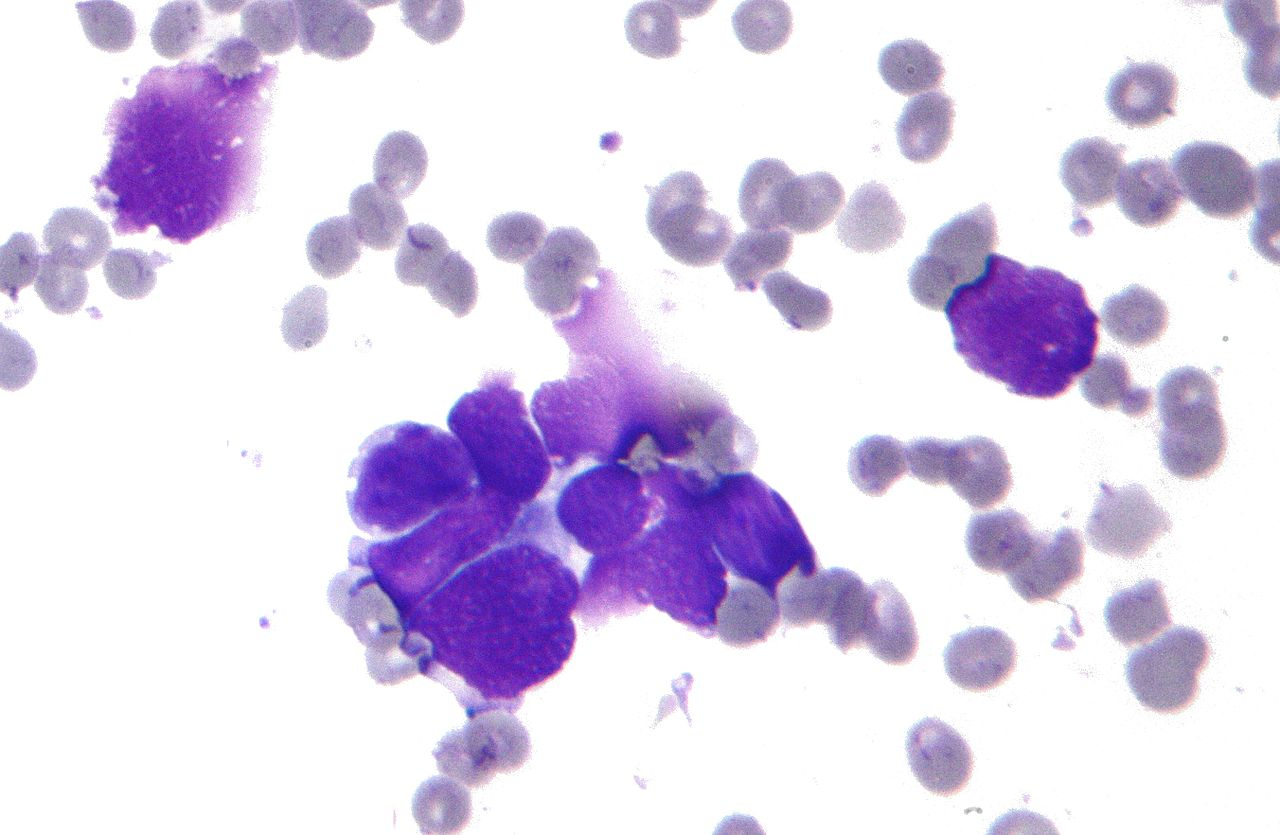
\includegraphics[width=25mm,height=20mm]{resources/carincomas}
        };
    \end{tikzpicture}%
    
    \begin{tikzpicture}[overlay,remember picture]
      \node[anchor=south east,xshift=-170pt,yshift=20pt]
        at (current page.south east) {
          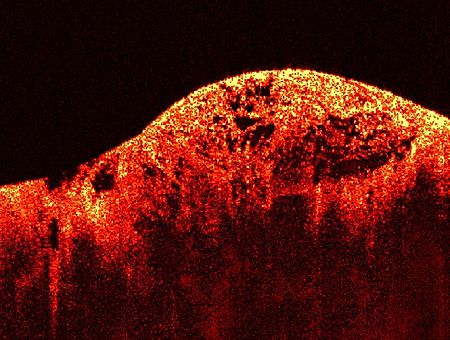
\includegraphics[width=25mm,height=20mm]{resources/sarcomas}
        };
    \end{tikzpicture}%
    
    \begin{tikzpicture}[overlay,remember picture]
      \node[anchor=south east,xshift=-90pt,yshift=20pt]
        at (current page.south east) {
          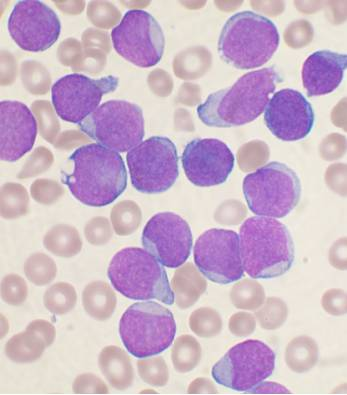
\includegraphics[width=25mm,height=20mm]{resources/leukemias}
        };
    \end{tikzpicture}%
    
    \begin{tikzpicture}[overlay,remember picture]
      \node[anchor=south east,xshift=-10pt,yshift=20pt]
        at (current page.south east) {
          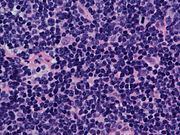
\includegraphics[width=25mm,height=20mm]{resources/lymphomas}
        };
    \end{tikzpicture}%
    \end{frame} 
    \begin{frame}[label=all]{Acute Lymphoblastic Leukemia}
      \begin{columns}
        \begin{column}{0.5\textwidth}
          Acute lymphocytic leukemia (ALL) is a type of cancer 
          of the blood and bone marrow, where blood cells are made. \\
           Normal lymphoblasts develop into mature, B-cells or T-cells.
           In ALL, both the normal development of some 
           lymphocytes and the control over the number of 
           lymphoid cells become defective.
        \end{column}
        \begin{column}{0.4\textwidth}
          \begin{figure}
            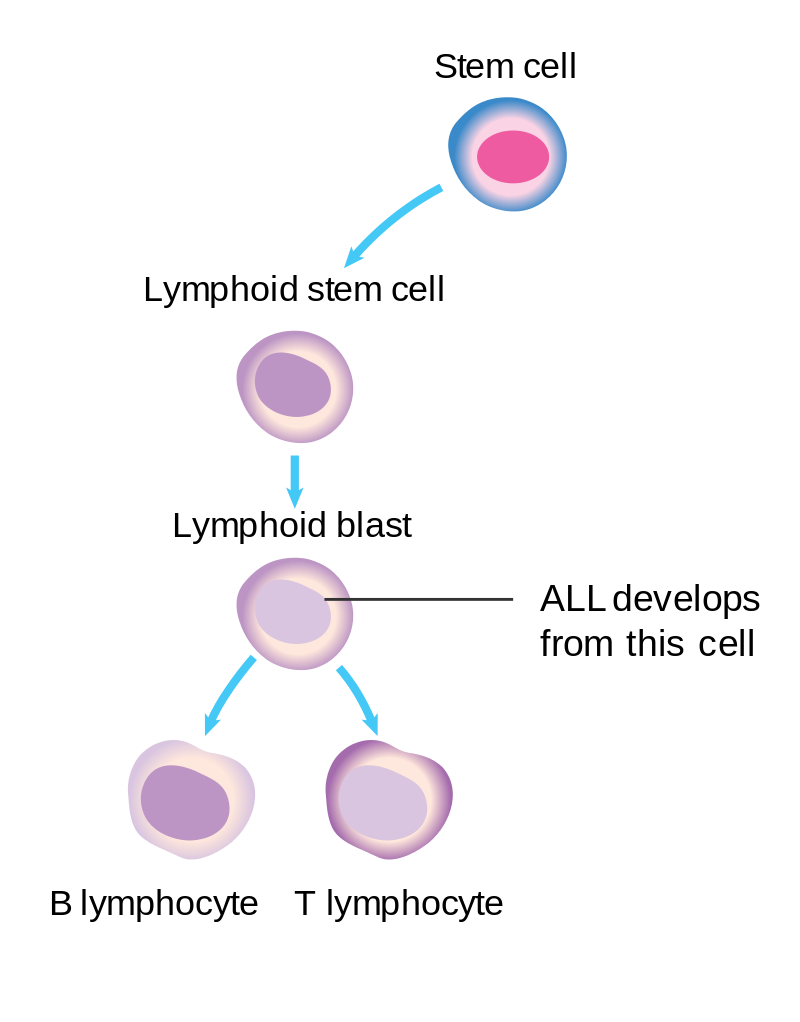
\includegraphics[width=\textwidth]{resources/all.png}
          \end{figure}
        \end{column}
      \end{columns}
    \end{frame}

    \section{Deep Learning Revisited: Cancer Detection}
    \subsection{Traditional Cancer Detection}
    \subsection{Deep Learning for Cancer Detection}
    \subsection{Practical Example}
    \subsection{Risks \& Warns}
    \begin{frame}
      test
    \end{frame}

\begin{frame}[label=bibliography]{Bibliography}
  \framesubtitle{\TeX, \LaTeX, and Beamer}
  \begin{thebibliography}{9}
    \bibitem{wikipedia}
    The free encyclopedia at
    \href{https://wikipedia.org}{wikipedia.org}
    \bibitem{handson}
    Hands-On Machine Learning with Scikit-Learn and TensorFlow: Concepts, Tools, and Techniques to Build Intelligent Systems
    \bibitem{dlb}
    Deep Learning (Ian J. Goodfellow, Yoshua Bengio and Aaron Courville), MIT Press, 2016.
    \bibitem{dlp}
    Deep Learning with Python (Francois Chollet), Manning Publications, 2017.
    \bibitem{cgov}
    National Cancer Institute, \href{https://www.cancer.gov}{www.cancer.gov}
    \bibitem{mayo}
    Mayo Clinic, \href{https://www.mayoclinic.org}{www.mayoclinic.org}
  \end{thebibliography}
\end{frame}

%   \section{Dark Frames}
%   \begin{darkframes}
%     \subsection{Blind Text}
%     \begin{frame}{Jabberwocky}
%       \framesubtitle{Lewis Carroll}%
%       \begin{tikzpicture}[overlay,remember picture]
%         \node[anchor=south east,xshift=-30pt,yshift=35pt]
%           at (current page.south east) {
%             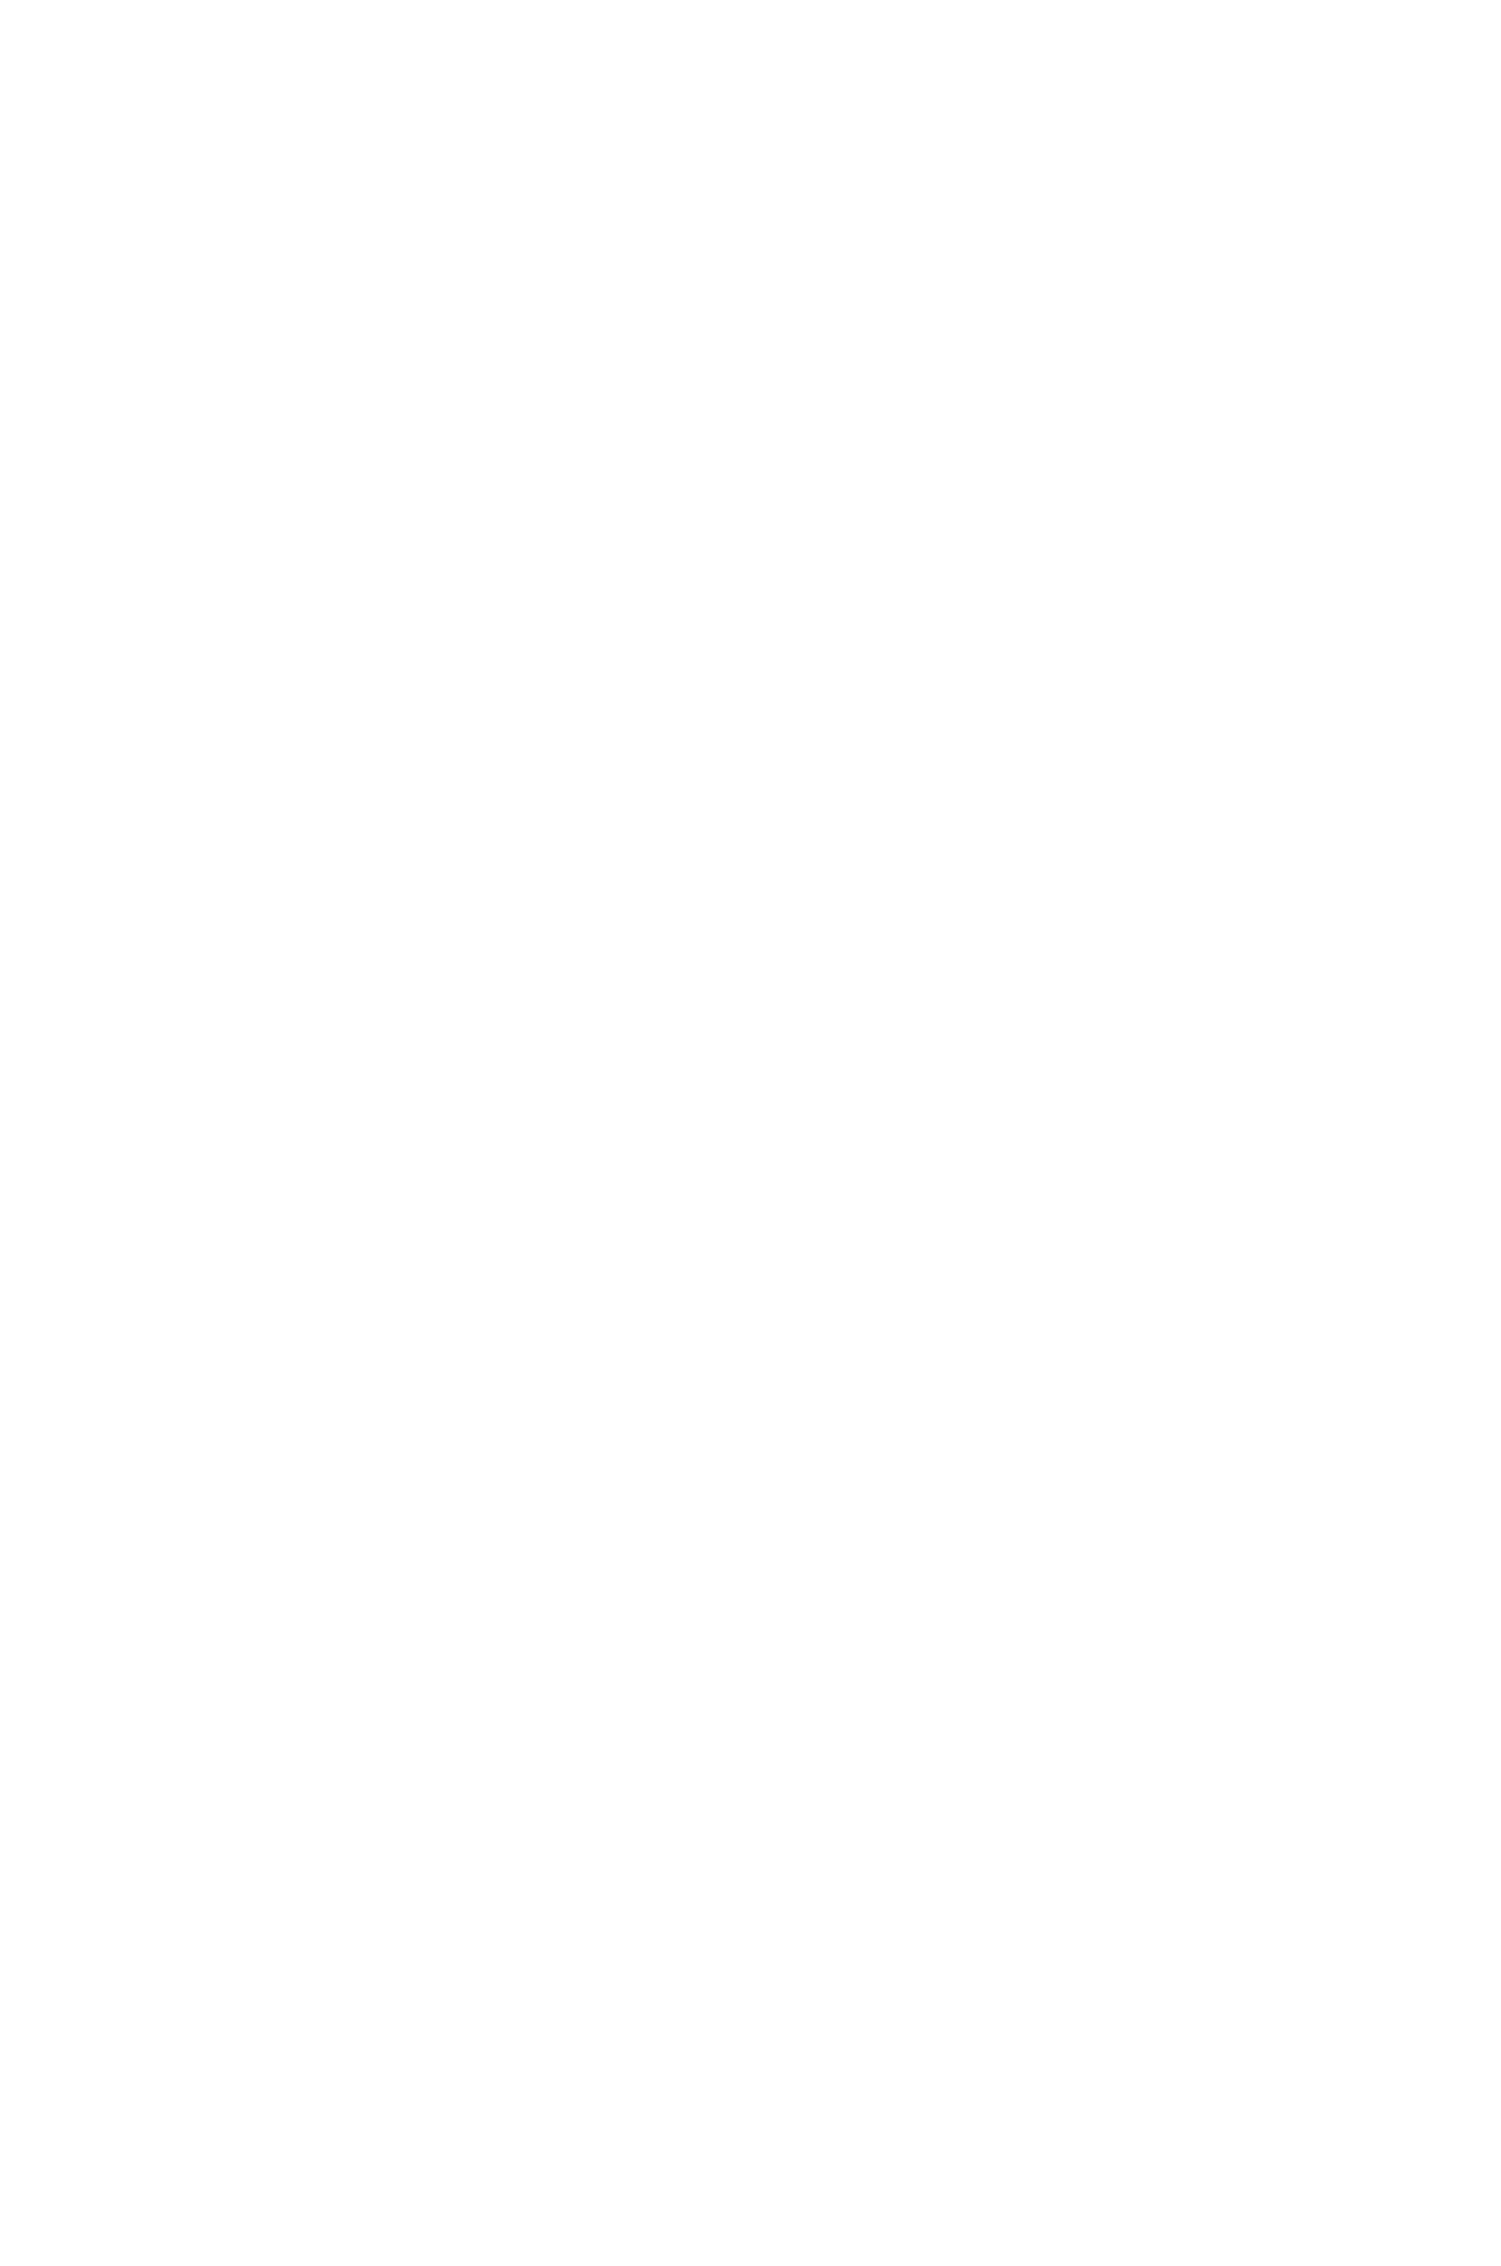
\includegraphics[width=35mm]{resources/jabberwocky-dark}
%           };
%       \end{tikzpicture}%
%       'Twas brillig, and the slithy toves\\
%       Did gyre and gimble in the wabe;\\
%       All mimsy were the borogoves,\\
%       And the mome raths outgrabe.\\\bigskip

%       “Beware the Jabberwock, my son!\\
%       The jaws that bite, the claws that catch!\\
%       Beware the Jubjub bird, and shun\\
%       The frumious Bandersnatch!”\\
%     \end{frame}
%     \againframe{lists}
%     \subsection{Structuring Elements}
%     \againframe{simmonshall}
%     \againframe{proof}
%     \subsection{Numerals and Mathematics}
%     \againframe{math}
%     \subsection{Figures and Code Listings}
%     \againframe{figs1}
%     \againframe{figs2}
%     \defverbatim[colored]\sleepSort{
%       \begin{lstlisting}[language=C,tabsize=2]
% #include <stdio.h>
% #include <unistd.h>
% #include <sys/types.h>
% #include <sys/wait.h>

% // This is a comment
% int main(int argc, char **argv)
% {
%         while (--c > 1 && !fork());
%         sleep(c = atoi(v[c]));
%         printf("%d\n", c);
%         wait(0);
%         return 0;
% }
%     \end{lstlisting}}
%   \begin{frame}{Code listings}{An example source code in C}
%       \sleepSort
%     \end{frame}
%     \subsection{Citations and Bibliography}
%     \againframe{citations}
%     \againframe{bibliography}
%   \end{darkframes}
\end{document}
